%!TEX TS-program = xelatex
%!TEX encoding = UTF-8 Unicode
%% Copyright 2011 Markus Gesmann

%\documentclass[a4paper,10pt,xetex]{article}
%\csname tex4ht\endcsname
\documentclass[11pt, twoside, openright, a4paper,xetex]{book}\usepackage[]{graphicx}\usepackage[]{color}
%% maxwidth is the original width if it is less than linewidth
%% otherwise use linewidth (to make sure the graphics do not exceed the margin)
\makeatletter
\def\maxwidth{ %
  \ifdim\Gin@nat@width>\linewidth
    \linewidth
  \else
    \Gin@nat@width
  \fi
}
\makeatother

\definecolor{fgcolor}{rgb}{0.345, 0.345, 0.345}
\newcommand{\hlnum}[1]{\textcolor[rgb]{0.686,0.059,0.569}{#1}}%
\newcommand{\hlstr}[1]{\textcolor[rgb]{0.192,0.494,0.8}{#1}}%
\newcommand{\hlcom}[1]{\textcolor[rgb]{0.678,0.584,0.686}{\textit{#1}}}%
\newcommand{\hlopt}[1]{\textcolor[rgb]{0,0,0}{#1}}%
\newcommand{\hlstd}[1]{\textcolor[rgb]{0.345,0.345,0.345}{#1}}%
\newcommand{\hlkwa}[1]{\textcolor[rgb]{0.161,0.373,0.58}{\textbf{#1}}}%
\newcommand{\hlkwb}[1]{\textcolor[rgb]{0.69,0.353,0.396}{#1}}%
\newcommand{\hlkwc}[1]{\textcolor[rgb]{0.333,0.667,0.333}{#1}}%
\newcommand{\hlkwd}[1]{\textcolor[rgb]{0.737,0.353,0.396}{\textbf{#1}}}%
\let\hlipl\hlkwb

\usepackage{framed}
\makeatletter
\newenvironment{kframe}{%
 \def\at@end@of@kframe{}%
 \ifinner\ifhmode%
  \def\at@end@of@kframe{\end{minipage}}%
  \begin{minipage}{\columnwidth}%
 \fi\fi%
 \def\FrameCommand##1{\hskip\@totalleftmargin \hskip-\fboxsep
 \colorbox{shadecolor}{##1}\hskip-\fboxsep
     % There is no \\@totalrightmargin, so:
     \hskip-\linewidth \hskip-\@totalleftmargin \hskip\columnwidth}%
 \MakeFramed {\advance\hsize-\width
   \@totalleftmargin\z@ \linewidth\hsize
   \@setminipage}}%
 {\par\unskip\endMakeFramed%
 \at@end@of@kframe}
\makeatother

\definecolor{shadecolor}{rgb}{.97, .97, .97}
\definecolor{messagecolor}{rgb}{0, 0, 0}
\definecolor{warningcolor}{rgb}{1, 0, 1}
\definecolor{errorcolor}{rgb}{1, 0, 0}
\newenvironment{knitrout}{}{} % an empty environment to be redefined in TeX

\usepackage{alltt} % twoside, openright
\usepackage{listings}	% you may not use this
\usepackage{algorithm2e} % you may not use this
\usepackage{banglatex}
\usepackage{setspace}
\usepackage[utf8]{inputenc}

%\usepackage[17pt]{extsizes} % to get fontsizes 8pt, 9pt, 10pt, 11pt, 12pt, 14pt, 17pt, 20pt through out the entire document.

% For BibLaTex
%\usepackage[backend=biber,style=alphabetic]{biblatex}
%\bibliography{sample}

\usepackage[colorlinks]{hyperref} %[,bookmarksopen]

\usepackage[none]{hyphenat}
\sloppy

\onehalfspacing
%\singlespacing
\IfFileExists{upquote.sty}{\usepackage{upquote}}{}
\begin{document}
%\title{ফলিত পরিসংখ্যান ও ডেটা সায়েন্স }
%\author{{\large নিউটন মু. আ. হাকিম}\\{\footnotesize mahnewton@dharapat.com}}
%\maketitle

%\newcommand{\ignore}[1]{}

%
%\tableofcontents
%\listoffigures
%\listoftables
%\listofalgorithms
%\lstlistoflistings

%for book the following things might help
\begin{titlepage}
	% design your title page here
	\Huge{ফলিত পরিসংখ্যান ও ডেটা সায়েন্স}
	
	\vspace{1in}
	
	\large{এনায়েতুর রহীম}
\end{titlepage}

\resetbengalipage
\bengalipageplainalpha
\tableofcontents
%\listoffigures
%\listoftables
%\listofalgorithms
%\lstlistoflistings
\clearpage
\resetbengalipage
\bengalipagefancynumber
\fancyhead[LO,RE]{\sl\nouppercase\leftmark} % twoside
\fancyhead[LE,RO]{\sl\nouppercase\rightmark} % twoside

% Input the introduction section

 % !Rnw root = PorishonkhanPorichiti.Rnw

\chapter{ভূমিকা}
এখানে ভূমিকা লিখতে হবে।

\section{পরিসংখ্যানে দক্ষতা অর্জন যে কারণে প্রয়োজন?}

লাইনের মাঝখানে  3.1415927  ধরে নেই $x=১০০ / ২০০$
 \[
 x = \frac{\sum(x_i)}{n} 
 \]
 একটি ড়্যান্ডম নাম্বার  0.1258534


"ড্যাটা ভিত্তিক সিদ্ধান্ত গ্রহণ" শব্দবন্ধটি কিছুদিন আগেও উন্নত বিশ্বে ব্যাপকভাবে আলোচিত হয়েছে। এখন সেখান থেকে আরো গভীরে গিয়ে আলোচিত হচ্ছে আর্টিফিশিয়াল ইন্টেলিজেন্স বা কৃত্রিম বুদ্ধিমত্তার ব্যবহার এবং কিভাবে ড্যাটা থেকে প্যাটার্ন বের করে তা সিদ্ধান্ত গ্রহণে কাজে লাগানো যায়। বলা হচ্ছে বিগ ডেটা ইজ বিগ ডিল। অনেক লেখালেখি হয়েছে বিগ ডেটা কিভাবে ব্যবসা বাণিজ্যকে বদলে দেবে এবং আগামী দিনে কারা প্রতিযোগিতায় টিকে থাকবে সেসব নিয়ে। বলা হচ্ছে যারা ডেটার সর্বোত্তম ব্যবহার করবে তারাই এগিয়ে যাবে কিংবা তাদেরই টিকে থাকার সম্ভাবনা বেশী হবে।

প্রশ্ন হলো এই প্রতিযোগিতায় আমরা কোথায় অবস্থান করছি। ব্যবসা বাণিজ্যে ডেটার ব্যবহার আমাদের দেশে সেভাবে এখনো শুরু না হলেও নিকট ভবিষ্যতে দ্রুত বেগে শুরু হবে বলে ধারণা করা যায়। বাংলাদেশে মোবাইলের ব্যবহার এবং মোবাইল ভিত্তিক সেবা যেমন-- ব্যাংকিং, এখন ব্যাপকভাবে প্রচলিত। এই ধারায় যুক্ত হচ্ছে মোবাইলে স্বাস্থ্য সেবা।
যদিও বাংলাদেশে ই-কমার্স সেভাবে বিস্তার লাভ করেনি যেভাবে এতদিনে বিস্তৃত হওয়ার কথা ছিল তবুও অল্পদিনের মধ্যেই ই-কমার্স জনপ্রিয় হবে বলে ধারণা করা যায়। কারণ এটি এখন সময়ের দাবি।
এখানে স্মরণ করা যেতে পারে বাংলাদেশের প্রথম ই-কমার্স সাইট মুনশিজি'র (munshigi.com) কথা। তখন ২০০২ বা  ২০০৩ সাল হবে। আমাজন ডট কম-এর পরিচিতির ঢেউ বাংলাদেশেও এসে পৌঁছেছিল। মুনশিজি মাঝখানে হারিয়ে গেলেও আবার ফিরে আসার প্রতিশ্রুতি দিচ্ছে।
আমরা বেশী দূরে না তাকিয়ে যদি ভারতের দিকেও তাকাই তাহলে দেখতে পাই ড্যাটাভিত্তিক সিদ্ধান্ত গ্রহণ করে অনেক ই-কমার্স স্টার-আপ কোম্পানি এই স্পেসে নিজেদের অবস্থান করে নিতে পেরেছে। অথচ বাংলাদেশে আমরা ই-কমার্স এখনো সেভাবে চালু করতে পারিনি। পারিন  এই নয় যে আমরা কখনোই পারবো না। বরং আগামীতে যা কিছু অগ্রগতি হবে তা হবে অসম্ভব দ্রুত গতিতে। এই গতি আনতেই হবে কারণ যারাই ধীরে চলবে তারাই পিছিয়ে পড়বে।
উন্নত বিশ্বে মার্কেটিং-এ এনালিটিক্স এর ব্যবহার হচ্ছে হরদম। কোন্ ধরনের ক্রেতার কাছে কোন্ ধরনের বিজ্ঞাপন পৌঁছাতে হবে সেটি নির্ধারণ করছে প্রেডিক্টিভ মডেল। এসব মডেল মেশিল লারনিং এ্যালগরিদম ব্যবহার করে ক্রেতাদের শ্রেনীভাগ করছে যাকে এরা বলে কাস্টমার সেগমেন্টেশন। বাংলাদেশে যখন পুরোদমে মার্কেটিং এনালিটিক্স শুরু হবে তখন পরিসংখ্যানবিদদের চাহিদা বাড়বে।
বাংলাদেশে যদিও অর্জিত জ্ঞান প্রয়োগের সুযোগ আগের দিনে অনেক সীমিত ছিল, ভবিষ্যতে তরুণ প্রজন্ম-দ্বারা পরিচালিত ব্যবসা বাণিজ্যে সাবজেক্টম্যাটার এক্সপার্ট তরুণরাই কাজ করবে বলে আমি মনে করি। এর কোন বিকল্প নেই।
আসছে দিনগুলোতে ড্যাটা ভিত্তিক সিদ্ধান্ত গ্রহণ এবং ব্যবসায় এনালিটিক্স-এর ব্যবহার বাড়বে। এ জন্য এসব ইন্ডাস্ট্রিতে দরকার হবে দক্ষ পরিসংখ্যানবিদ এবং ড্যাটা সাইন্টিস্ট। ড্যাটা সাইন্টিস্ট হওয়ার জন্য পরিসংখ্যানবিদ হওয়ার প্রয়োজন নেই তবে পরিসংখ্যানবিদদের জন্য ড্যাটা সাইন্টিস্ট-হওয়া অনেকটা সহজ। কারণ ড্যাটা সাইন্টিস্ট হলো পরিসংখ্যান, কম্পিউটার প্রোগ্রামিং, শৈল্পিক আইডিয়া এবং বিষয়ভিত্তিক জ্ঞান-এসবের সমাহার।
পরিসংখ্যানের ছাত্রছাত্রীরা এই দৌড়ে অনেকটাই এগিয়ে থাকবে। তবে এগিয়ে থাকবে সেই আনন্দে বসে থাকলে চলবে না। উৎসাহী এবং পরিশ্রমী যে কেউই এই দৌড়ে জয়ের সামর্থ রাখে। যারা পরিসংখ্যানের ছাত্রছাত্রী, তাদেরকে পরিসংখ্যান ব্যবহার করার চর্চা করে যেতে হবে। অর্থাৎ শুধু প্রথাগত জ্ঞান অর্জন নয়, সেই অর্জিত জ্ঞানের ব্যবহার করা শিখতে হবে।
কিন্তু বাংলাদেশে তো সেভাবে কিছু করার সুযোগ নেই! সেটা সত্যি। তবে এ জন্য তো আর আত্মউন্নয়নকে বসিয়ে রাখা যাবে না। ইন্টারনেটের যুগে এখন সব জ্ঞান হাতের মুঠোয়। দরকার একটুখানি সদিচ্ছা, নিরলস প্রচেষ্টা আর অধ্যাবসায়।
একটা বিষয় আমাকে আশাবাদী করে যখন দেখি আমাদের ছাত্র-ছাত্রীরা পরিসংখ্যানে পড়াশুনা করছে এবং তাদের মধ্যে অল্প কয়েকজন বাদে সবাই ডিগ্রী শেষ করছে। স্নাতক পর্যায়ে আমাদের প্রতিটি পাবলিক বিশ্ববিদ্যালয়েই পরিসংখ্যান পড়ানো হয়। সে হিসেবে প্রতি বছর আনুমানিক ২-৪শ’র মতো ছাত্রছাত্রী পরিসংখ্যানে স্নাতক অর্জন করে। সংখ্যাটি একেবারে কম নয়।
আমাদের দেশের শিক্ষা ব্যবস্থার একটা বড় সীমাবদ্ধতা হলো অর্জিত শিক্ষাকে কর্মক্ষেত্রে প্রয়োগ করার পরিসর অনেক ছোট। অধিকাংশ ক্ষেত্রেই তা অনুপস্থিত। যদিও বিসিএস ক্যাডারে পরিসংখ্যানের একটা ক্যাডার আছে, কিন্তু সেটি প্রকৃতপক্ষে পরিসংখ্যানের ছাত্রছাত্রীদের খুব একটা আকৃষ্ট করে বলে আমার মনে হয়নি কখনো। বাস্তবতার নিরীখে বলা যায় অধিকাংশ ক্ষেত্রেই অন্যান্য বিষয়ের মতো পরিসংখ্যানের ছাত্র-ছাত্রীরাও সম্পূর্ণ ভিন্ন কোন ফিল্ডে কর্মজীবন শুরু করে।
আমার স্বল্প অভিজ্ঞতায় দেখেছি যারা বিশ্ববিদ্যালয় পর্যায়ে ভালো ফলাফল করে অর্থাৎ প্রথম শ্রেনীতে উপরের দিকে অবস্থান করে বা জিপিএ ৩.৮ বা তার উপরে থাকে, তারা শিক্ষকতাকে পেশা হিসেবে বেছে নেয়। অন্যভাবে বলা যায় তাদের জন্য পরিসংখ্যানের সাথে জড়িয়ে থাকাটা বেশ খানিকটা সহজ হয়।
অল্প সংখ্যক পরিসংখ্যানবিদদের পরিসংখ্যান নিয়ে কাজ করার সুযোগ থাকলেও একটা বিরাট অংশই পরিসংখ্যান থেকে দূরে সরে যায়। এটি প্রকৃতপক্ষে সময় এবং মেধার এক বিশাল অপচয়। এই বিরাট অংশের ভগ্নাংশও যদি পরিসংখ্যানের সাথে সম্পৃক্ত রাখা যেতো তাহলে এদের মধ্যেই অনেকেই অনেক ভালো করতো বলে আমি বিশ্বাস করি।
এই অপচয় রোধ করার সহজ কোন উপায় নেই যা দেশে ব্যক্তিপর্যায়ে সৃষ্টি করা যায়। অথচ উন্নত বিশ্বে পরিসংখ্যানবিদদের ঘাটতি হবে বলে নানা গবেষণায় দেখানো হচ্ছে।
গ্লোবালাইজেশনের যুগে সেদিন দূরে নয় হয়তো বাংলাদেশে বসেই পরিসংখ্যানবিদগণ আমেরিকার কোন একটি কোম্পানীর কাজ করে দিবে। ভারত সেটি বাস্তবায়ন করতে পেরেছে। আমরা ভারতের চেয়ে এদিক থেকে অন্তত ৪/৫ বছর পিছিয়ে আছি। তবে আশার কথা সরকার এখন আইটি-ক্ষেত্রে অনেক জোর দিচ্ছে। এই ধারা অব্যাহত থাকলে নিকট ভবিষ্যতে আমরাও পারবো এনালিটিক কাজগুলো দেশ থেকে সম্পন্ন করতে।
এই যাত্রায় অভিযাত্রী হতে পরিসংখ্যানের গুরুত্ব অপরিসীম। বলা যায় পরিসংখ্যান ব্যতীত এ যাত্রায় কোন ফল আশা করা অসম্ভব।  সে কারণে পরিসংখ্যান সম্পর্কে বেসিক ধারণা কমবেশী সবারই থাকা প্রয়োজন।
 
পরিসংখ্যান কী?

পাই এর মান আমরা জানি 3.14.

\begin{knitrout}
\definecolor{shadecolor}{rgb}{0.969, 0.969, 0.969}\color{fgcolor}\begin{kframe}
\begin{alltt}
\hlkwd{set.seed}\hlstd{(}\hlnum{1213}\hlstd{)}  \hlcom{# for reproducibility}
\hlstd{x} \hlkwb{=} \hlkwd{cumsum}\hlstd{(}\hlkwd{rnorm}\hlstd{(}\hlnum{100}\hlstd{))}
\hlkwd{mean}\hlstd{(x)}  \hlcom{# mean of x}
\end{alltt}
\begin{verbatim}
## [1] -1.939758
\end{verbatim}
\begin{alltt}
        \hlkwd{plot}\hlstd{(x,} \hlkwc{type} \hlstd{=} \hlstr{'l'}\hlstd{)}  \hlcom{# Brownian motion}
\end{alltt}
\end{kframe}
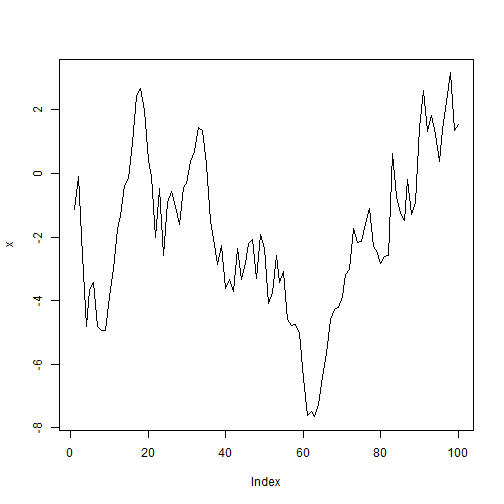
\includegraphics[width=\maxwidth]{figure/my-label-1} 

\end{knitrout}

আমাদের একটা ধারণা রয়েছে যে পরিসংখ্যান মানেই সারণি আর সংখ্যা। সেটি অবশ্য ভুল নয়। কিন্তু এটি পরিসংখ্যানের অতি ক্ষুদ্র একটি অংশ মাত্র। এটি ঠিক যে পরিসংখ্যানের প্রাথমিক কাজই হলো উপাত্ত থেকে তথ্য বের করে আনা। লক্ষ্য করুন আমি বলেছি উপাত্ত থেকে তথ্য বের করার কথা। আপাতদৃস্টিতে উপাত্ত আর তথ্য অনেকের কাছে সমার্থক মনে হতে পারে। কিন্তু আমাদের জানতে হবে এদের পার্থক্য কোথায়।
ধরা যাক গত বিশ বছরের স্যাটেলাইট ইমেজিং এর মাধ্যমে বাংলাদেশের দক্ষিণাঞ্চলের বনভূমির চিত্র সংগ্রহ করা হয়েছে। এই চিত্রগুলো এবং আনুষংজ্ঞিক যে ডেটা সংগ্রহ করা হয়েছে সেগুলো শুধুই ডেটা বা উপাত্ত। কিন্তু এই ডেটাকে বিশ্লেষণ করে যখন দেখা যাবে বিশ বছর আগে আমাদের যে পরিমাণ বনভূমি ছিল আজকে তার চেয়ে অনেক কম বনভূমি অবশিষ্ট রয়েছে তখন এটিকে আমরা বলব তথ্য। উপাত্ত থাকলেই সেটি এমনি এমনি কাজের হবে এমনটি নয়। বরং সেটিকে কাজের উপযোগী করা পরিসংখ্যানের অন্যতম কাজ। অবশ্যই উপাত্ত সংগ্রহ এবং তার পরিকল্পনাও পরিসংখ্যানের অংশ।
তাহলে দেখা গেল উপাত্ত মানেই তথ্য নয়। উপাত্তকে বরং খনি থেকে প্রাপ্ত আকরিকের সাথে তুলনা করা যায়। আকরিককে যেমন নানা প্রক্রিয়ার মধ্যে দিয়ে তা থেকে লোহা বের করা হয়। তেমনি  উপাত্তকে ধুয়ে মুছে পরিস্কার করে তা থেকে তথ্য বের করে আনাই পরিসংখ্যানের উদ্দেশ্য। আর সেজন্য যেসব উপকরণ ও পদ্ধতির প্রয়োজন তা আমরা পরিসংখ্যান নামক আপাত: ভীতিকর বিষয় থেকে জানতে পারবো।

উইকিপিডিয়া থেকে- ``Statistics is the study of the collection, organization, analysis, interpretation, and presentation of data. It deals with all aspects of this, including the planning of data collection in terms of the design of surveys and experiments.''

এই সংজ্ঞা থেকে পরিসংখ্যানের একটি দিক সম্পর্কে আমরা ধারনা পাই। সেটি হলো উপাত্তের বিশ্লেষণ, ব্যাখ্যা ও পরিবেশন সম্পর্কিত। পরিসংখ্যানের এই দিকটিকে বলা হয় বর্ণনামূলক পরিসংখ্যান বা ডেসক্রিপটিভ পরিসংখ্যান। এই সংজ্ঞায় পরিসংখ্যানের (আমার মতে) সবচেয়ে গুরুত্বপূর্ণ দিকটিই না বলা রয়ে গেছে। সেটি হলো – সিদ্ধান্ত গ্রহণে পরিসংখ্যানের ব্যবহার এবং সে সম্পর্কিত দিকটি যাকে ইংরেজীতে আমরা বলি ইনফারেনসিয়াল পরিসংখ্যান। পরিসংখ্যানের যে অংশটি পরিশোধিত উপাত্ত (তথ্য)-কে ব্যবহার করে প্রকল্পের পরীক্ষণ (টেস্ট অব হাইপোথিসিস) করে এবং তা থেকে সিদ্ধান্ত গ্রহণে (ডিসিসন মেকিং) ভূমিকা রাখে সেই অংশটিকে বলে ইনফারেনসিয়াল পরিসংখ্যান।

%\SweaveInput{introduction.Rnw}



% \include{introduction}
%\input{probability_distribution}
%\input{sampling_distribution}

% For BibTeX
\bibliographystyle{plain} %plain
\bibliography{sample}

%For BibLaTeX
%\printbibliography

% Issue to be fixed.

%A sample code inclusion command: \lstinputlisting[label={code:simple-code},caption={simple code.cpp}]{code/chapter_2/simple_code.cpp}, and corresponding reference command is: \ref{code:simple-code}
\end{document}

